\documentclass[12pt,a4paper]{article}

% Codificación e idioma
\usepackage[utf8]{inputenc}
\usepackage[T1]{fontenc}
\usepackage[spanish,es-nodecimaldot]{babel}
\usepackage{lmodern}

% Diseño de página
\usepackage[a4paper,margin=2.5cm,headheight=15pt]{geometry}
\usepackage{setspace}
\usepackage{fancyhdr}
\usepackage{parskip}
\usepackage{enumitem}

% Tablas y figuras
\usepackage{array}
\usepackage{booktabs}
\usepackage{longtable}
\usepackage{tabularx}
\usepackage{ragged2e}
\usepackage{graphicx}
\graphicspath{{docs/}{./}}
\usepackage{float}
\usepackage{tikz}
\usetikzlibrary{arrows.meta,positioning,shapes.geometric,fit}

% Código, colores y enlaces
\usepackage{xcolor}
\usepackage{listings}
\usepackage{hyperref}
\usepackage{microtype}

\definecolor{uaiBlue}{HTML}{17365D}
\definecolor{techBlue}{HTML}{2F5597}
\definecolor{lightBlue}{HTML}{D9EAF7}
\definecolor{lightGray}{HTML}{F2F2F2}
\definecolor{darkGray}{HTML}{404040}
\definecolor{codeGreen}{HTML}{2E7D32}

\hypersetup{
    colorlinks=true,
    linkcolor=uaiBlue,
    urlcolor=techBlue,
    citecolor=uaiBlue,
    pdftitle={Análisis Técnico del Sistema de Gestión de Ventas},
    pdfauthor={Ruffinengo Yasmin, Noya Ana y Civilotti Genaro},
    pdfsubject={Trabajo final - TechStore S.A.}
}

\pagestyle{fancy}
\fancyhf{}
\lhead{\small Universidad Abierta Interamericana}
\rhead{\small TechStore S.A.}
\cfoot{\thepage}

\setstretch{1.15}
\setlength{\parindent}{0pt}
\setlist[itemize]{topsep=4pt,itemsep=2pt}
\setlist[enumerate]{topsep=4pt,itemsep=2pt}

\newcolumntype{Y}{>{\RaggedRight\arraybackslash}X}
\newcolumntype{L}[1]{>{\RaggedRight\arraybackslash}p{#1}}

\lstdefinestyle{csharp}{
    language=[Sharp]C,
    basicstyle=\ttfamily\small,
    keywordstyle=\color{techBlue}\bfseries,
    commentstyle=\color{codeGreen},
    stringstyle=\color{red!60!black},
    backgroundcolor=\color{lightGray},
    frame=single,
    rulecolor=\color{gray!50},
    breaklines=true,
    showstringspaces=false,
    tabsize=4,
    columns=fullflexible
}

\tikzset{
    component/.style={
        rectangle,
        rounded corners,
        draw=techBlue,
        very thick,
        fill=lightBlue,
        align=center,
        minimum width=3.2cm,
        minimum height=1.25cm,
        text width=3cm
    },
    external/.style={
        cylinder,
        shape border rotate=90,
        aspect=0.25,
        draw=darkGray,
        very thick,
        fill=lightGray,
        align=center,
        minimum width=2.8cm,
        minimum height=1.3cm
    },
    flow/.style={
        rectangle,
        rounded corners,
        draw=techBlue,
        thick,
        fill=lightBlue,
        align=center,
        text width=5.3cm,
        minimum height=0.9cm
    },
    decision/.style={
        diamond,
        draw=darkGray,
        thick,
        fill=lightGray,
        align=center,
        aspect=2.4,
        text width=3.2cm
    },
    arrow/.style={-{Latex[length=3mm]},thick,draw=darkGray}
}

\begin{document}

% ---------------------------------------------------------------------------
% Portada
% ---------------------------------------------------------------------------
\begin{titlepage}
    \centering

    \vspace*{1.5cm}

    {\Large\bfseries\color{uaiBlue}
    Universidad Abierta Interamericana\par}

    \vspace{2.2cm}

    {\large Trabajo Final\par}
    \vspace{0.4cm}
    {\Huge\bfseries Sistema de Gestión de Ventas\par}
    \vspace{0.6cm}
    {\LARGE TechStore S.A.\par}

    \vspace{1.8cm}

    \rule{0.75\textwidth}{1.2pt}
    \vspace{0.5cm}

    {\LARGE\bfseries\color{techBlue} Análisis Técnico\par}

    \vspace{0.5cm}
    \rule{0.75\textwidth}{1.2pt}

    \vfill

    {\large\bfseries Alumnos\par}
    \vspace{0.5cm}

    {\large
    Ruffinengo Yasmin\par
    Noya Ana\par
    Civilotti Genaro\par}

    \vfill

    {\large Julio de 2026\par}

    \vspace{1cm}
\end{titlepage}

\tableofcontents
\newpage

% ---------------------------------------------------------------------------
\section{Propósito y alcance}

Este documento describe y justifica la arquitectura implementada para el
Sistema de Gestión de Ventas de TechStore S.A. El análisis se basa en la
solución desarrollada y cubre:

\begin{itemize}
    \item la arquitectura general y la aplicación del patrón MVC;
    \item los patrones de diseño utilizados y los recomendados para evolucionar
    el sistema;
    \item la estrategia de integración entre la interfaz, la lógica de negocio,
    la persistencia, SQL Server y el servicio externo de facturación;
    \item el tratamiento de transacciones, validaciones, errores, configuración
    y seguridad;
    \item la trazabilidad de los requerimientos;
    \item los riesgos técnicos, las limitaciones actuales y las mejoras
    propuestas;
    \item la estrategia de pruebas y despliegue.
\end{itemize}

La solución es una aplicación de escritorio para Windows desarrollada con
.NET y Windows Forms. La persistencia se realiza en SQL Server mediante Entity
Framework Core con un enfoque Code First.

% ---------------------------------------------------------------------------
\section{Resumen de la solución}

La solución está organizada en cuatro proyectos:

\begin{table}[H]
\centering
\caption{Proyectos y responsabilidades}
\begin{tabularx}{\textwidth}{L{2.8cm} L{3.5cm} Y}
\toprule
\textbf{Proyecto} & \textbf{Rol arquitectónico} &
\textbf{Responsabilidad principal} \\
\midrule
\texttt{Vista} & Vista &
Formularios, grillas, captura de datos, navegación y presentación de mensajes. \\
\texttt{Controladora} & Controlador / aplicación &
Validaciones, coordinación de casos de uso, cálculos y reglas de negocio. \\
\texttt{Modelo} & Acceso a datos e integración &
Repositorios, consultas LINQ, transacciones, contexto de EF Core, migraciones
y carga de configuración. \\
\texttt{Entidades} & Modelo de dominio y contratos &
Entidades, relaciones, enumeraciones y DTO utilizados por reportes y consultas. \\
\bottomrule
\end{tabularx}
\end{table}

\subsection{Vista general de la arquitectura}

\begin{figure}[H]
\centering
\resizebox{\textwidth}{!}{%
\begin{tikzpicture}[node distance=1.25cm and 1.5cm]
    \node[component] (user) {Usuario};
    \node[component, right=of user] (view) {Vista\\Windows Forms};
    \node[component, right=of view] (controller)
        {Controladora\\Casos de uso y reglas};
    \node[component, below=of controller] (model)
        {Modelo\\Repositorios y EF Core};
    \node[component, below=of view] (entities)
        {Entidades\\Dominio y DTO};
    \node[external, right=of model] (db) {SQL Server};
    \node[component, above=of controller] (invoice)
        {API externa\\de facturación};

    \draw[arrow] (user) -- (view);
    \draw[arrow] (view) -- (controller);
    \draw[arrow] (controller) -- (model);
    \draw[arrow] (controller) -- (entities);
    \draw[arrow] (model) -- (entities);
    \draw[arrow] (model) -- (db);
    \draw[arrow] (controller) -- node[right,align=left,font=\small]
        {JSON / PDF} (invoice);
\end{tikzpicture}
}
\caption{Arquitectura general del sistema}
\end{figure}

En la implementación actual, \texttt{Vista} también referencia
\texttt{Modelo} para cargar el archivo de configuración y comprobar la conexión
durante el inicio. Esta dependencia funciona, pero sería conveniente
encapsularla en un servicio de inicialización para mantener más estrictamente
el límite entre capas.

% ---------------------------------------------------------------------------
\section{Decisiones arquitectónicas}

\subsection{Arquitectura en capas}

La separación en proyectos reduce el acoplamiento entre interfaz, reglas y
persistencia. Una modificación visual no debería cambiar las consultas a la
base de datos; del mismo modo, un cambio de persistencia debería afectar
principalmente al proyecto \texttt{Modelo}.

Las dependencias deben apuntar hacia el dominio:

\begin{enumerate}
    \item \texttt{Vista} conoce a \texttt{Controladora} y \texttt{Entidades}.
    \item \texttt{Controladora} conoce a \texttt{Modelo} y \texttt{Entidades}.
    \item \texttt{Modelo} conoce a \texttt{Entidades} y a Entity Framework Core.
    \item \texttt{Entidades} no debería depender de la interfaz ni de la base
    de datos.
\end{enumerate}

Esto favorece la mantenibilidad solicitada, aunque todavía existe margen para
mejorar mediante interfaces e inyección de dependencias.

\subsection{MVC adaptado a una aplicación de escritorio}

El patrón MVC se aplica de la siguiente manera:

\begin{table}[H]
\centering
\small
\caption{Correspondencia entre MVC y la solución}
\begin{tabularx}{\textwidth}{L{2.5cm} Y L{4.2cm}}
\toprule
\textbf{Elemento MVC} & \textbf{Implementación} & \textbf{Ejemplos} \\
\midrule
Modelo &
Entidades del dominio y repositorios de persistencia. &
\texttt{Venta}, \texttt{Producto}, \texttt{Inventario},
\texttt{Repositorio\allowbreak Venta}. \\
Vista &
Formularios Windows Forms. &
\texttt{frmVenta}, \texttt{frmProducto},
\texttt{frmReporte\allowbreak Venta}. \\
Controlador &
Clases que reciben las solicitudes de la Vista y coordinan reglas y
repositorios. &
\texttt{Controladora\allowbreak Venta},
\texttt{Controladora\allowbreak Producto},
\texttt{Controladora\allowbreak Reporte}. \\
\bottomrule
\end{tabularx}
\normalsize
\end{table}

Por ejemplo, la vista de ventas captura la selección del cliente, la sucursal,
el vendedor, el método de pago y los productos, y construye una entidad
\texttt{Venta}. Después, la controladora correspondiente valida y calcula los
importes y delega la persistencia al repositorio de ventas.

% ---------------------------------------------------------------------------
\section{Patrones implementados}

En la solución se incluyen patrones arquitectónicos y de persistencia que resuelven problemas comunes y cuya aplicación nos otorga diversos beneficios

\subsection{Modelo--Vista--Controlador}

\textbf{Problema resuelto.} Evitar que presentación, reglas de negocio y
acceso a datos queden mezclados en los formularios.

\textbf{Aplicación.} Los formularios representan la Vista; las entidades y
repositorios forman el Modelo; y las controladoras coordinan las operaciones.

\textbf{Beneficio.} Permite modificar la interfaz o las reglas con menor
impacto sobre el resto del sistema y asignar responsabilidades claras a los
integrantes.

\subsection{Singleton}

\textbf{Problema resuelto.} Brindar un punto de acceso único a cada
controladora desde los distintos formularios.

\textbf{Aplicación.} Las controladoras exponen una propiedad estática
\texttt{Instancia} y mantienen su constructor privado.

\textbf{Beneficio.} Simplifica el acceso y evita crear repetidamente objetos
coordinadores.

\textbf{Costo.} Introduce estado global y dependencias ocultas, dificulta las
pruebas aisladas y la ejecución concurrente. Es aceptable para el alcance
académico y el proceso único de escritorio, pero para una evolución productiva
se recomienda sustituirlo por inyección de dependencias con un ciclo de vida
controlado.

\subsection{Data Mapper y ORM}

\textbf{Problema resuelto.} Traducir entre objetos C\# y tablas relacionales.

\textbf{Aplicación.} Entity Framework Core mapea entidades, claves, relaciones
e índices mediante \texttt{DbContext} y Fluent API.

\textbf{Beneficio.} Permite expresar consultas con LINQ, administrar relaciones
y versionar el esquema mediante migraciones.

% ---------------------------------------------------------------------------

\section{Estrategia de integración entre componentes}

\subsection{Integración interna}

La integración entre los proyectos es directa, en memoria y sin serialización:

\begin{enumerate}
    \item La Vista captura y valida datos de formato básico.
    \item La Vista crea entidades o parámetros de consulta.
    \item La Controladora valida reglas de negocio y coordina el caso de uso.
    \item El Repositorio traduce la operación a consultas y comandos de EF Core.
    \item EF Core ejecuta SQL parametrizado sobre SQL Server.
    \item El resultado retorna como entidad, colección de sólo lectura, DTO o
    mensaje de operación.
\end{enumerate}

Las entidades se utilizan en operaciones transaccionales y los DTO en consultas
preparadas para presentación.

\subsection{Integración con SQL Server}

\texttt{Context} deriva de \texttt{DbContext} y expone un \texttt{DbSet} por
agregado persistente. La cadena de conexión se obtiene desde
\texttt{DB\_DSN}; no se encuentra escrita en el código.

Las consultas de lectura usan mayormente \texttt{AsNoTracking}, lo que reduce
el costo del seguimiento cuando el resultado no va a modificarse. Para la
venta, el contexto sí mantiene seguimiento del inventario porque debe detectar
y persistir la disminución del stock.

Las migraciones permiten:

\begin{itemize}
    \item crear el esquema inicial;
    \item reproducir relaciones, índices y datos iniciales;
    \item incorporar de forma versionada la cuenta corriente;
    \item mantener alineadas las instalaciones de todos los integrantes.
\end{itemize}

\subsection{Integración con el servicio de facturación}

La generación del comprobante sigue este flujo:

\begin{enumerate}
    \item El usuario selecciona una venta ya registrada.
    \item La Vista solicita a \texttt{ControladoraVenta} la venta completa con
    cliente, método de pago, detalle y productos.
    \item \texttt{ControladoraFactura} transforma la venta en el contrato JSON
    externo.
    \item Envía una solicitud \texttt{POST} autenticada con Bearer token.
    \item Solicita y valida una respuesta \texttt{application/pdf}.
    \item Retorna los bytes del PDF a la Vista.
    \item La Vista guarda el archivo en la ubicación elegida por el usuario.
\end{enumerate}

La URL y la clave se leen desde \texttt{FACTURACION\_API\_URL} y
\texttt{FACTURACION\_API\_KEY}.

\begin{figure}[H]
\centering
\begin{tikzpicture}[node distance=0.7cm]
    \node[flow] (a) {El usuario selecciona una venta};
    \node[flow, below=of a] (b)
        {\texttt{ControladoraVenta} obtiene la venta y sus relaciones};
    \node[flow, below=of b] (c)
        {\texttt{ControladoraFactura} construye el contrato JSON};
    \node[flow, below=of c] (d)
        {Solicitud HTTP POST con Bearer token};
    \node[flow, below=of d] (e)
        {La API externa genera y devuelve el PDF};
    \node[flow, below=of e] (f)
        {La Vista guarda el comprobante};

    \draw[arrow] (a) -- (b);
    \draw[arrow] (b) -- (c);
    \draw[arrow] (c) -- (d);
    \draw[arrow] (d) -- (e);
    \draw[arrow] (e) -- (f);
\end{tikzpicture}
\caption{Flujo de integración con el servicio de facturación}
\end{figure}

La llamada es asíncrona para no bloquear la interfaz. Se reutiliza una instancia
estática de \texttt{HttpClient}, evitando el agotamiento de conexiones.

\subsection{Integración de reportes}

Los filtros se reciben en la controladora y se componen en el repositorio
mediante LINQ. Entity Framework traduce agrupaciones, sumas, filtros y
proyecciones a SQL para que el procesamiento ocurra en la base de datos.

Para incluir el día final completo se utiliza un intervalo semiabierto:

\begin{lstlisting}[style=csharp,caption={Tratamiento del rango de fechas}]
FechaVenta >= fechaDesde.Date
FechaVenta < fechaHasta.Date.AddDays(1)
\end{lstlisting}

Esta forma evita problemas producidos por componentes de hora, minutos y
segundos.

% ---------------------------------------------------------------------------
\clearpage
\section{Diagrama de clases}
\thispagestyle{fancy}

El siguiente diagrama representa las entidades persistentes del sistema, sus
atributos principales, claves primarias y foráneas, enumeraciones, clases
asociativas y multiplicidades. Los DTO utilizados por los reportes no se
incluyen porque son proyecciones de consulta y no forman parte del modelo de
dominio persistente.

\begin{figure}[H]
    \centering
    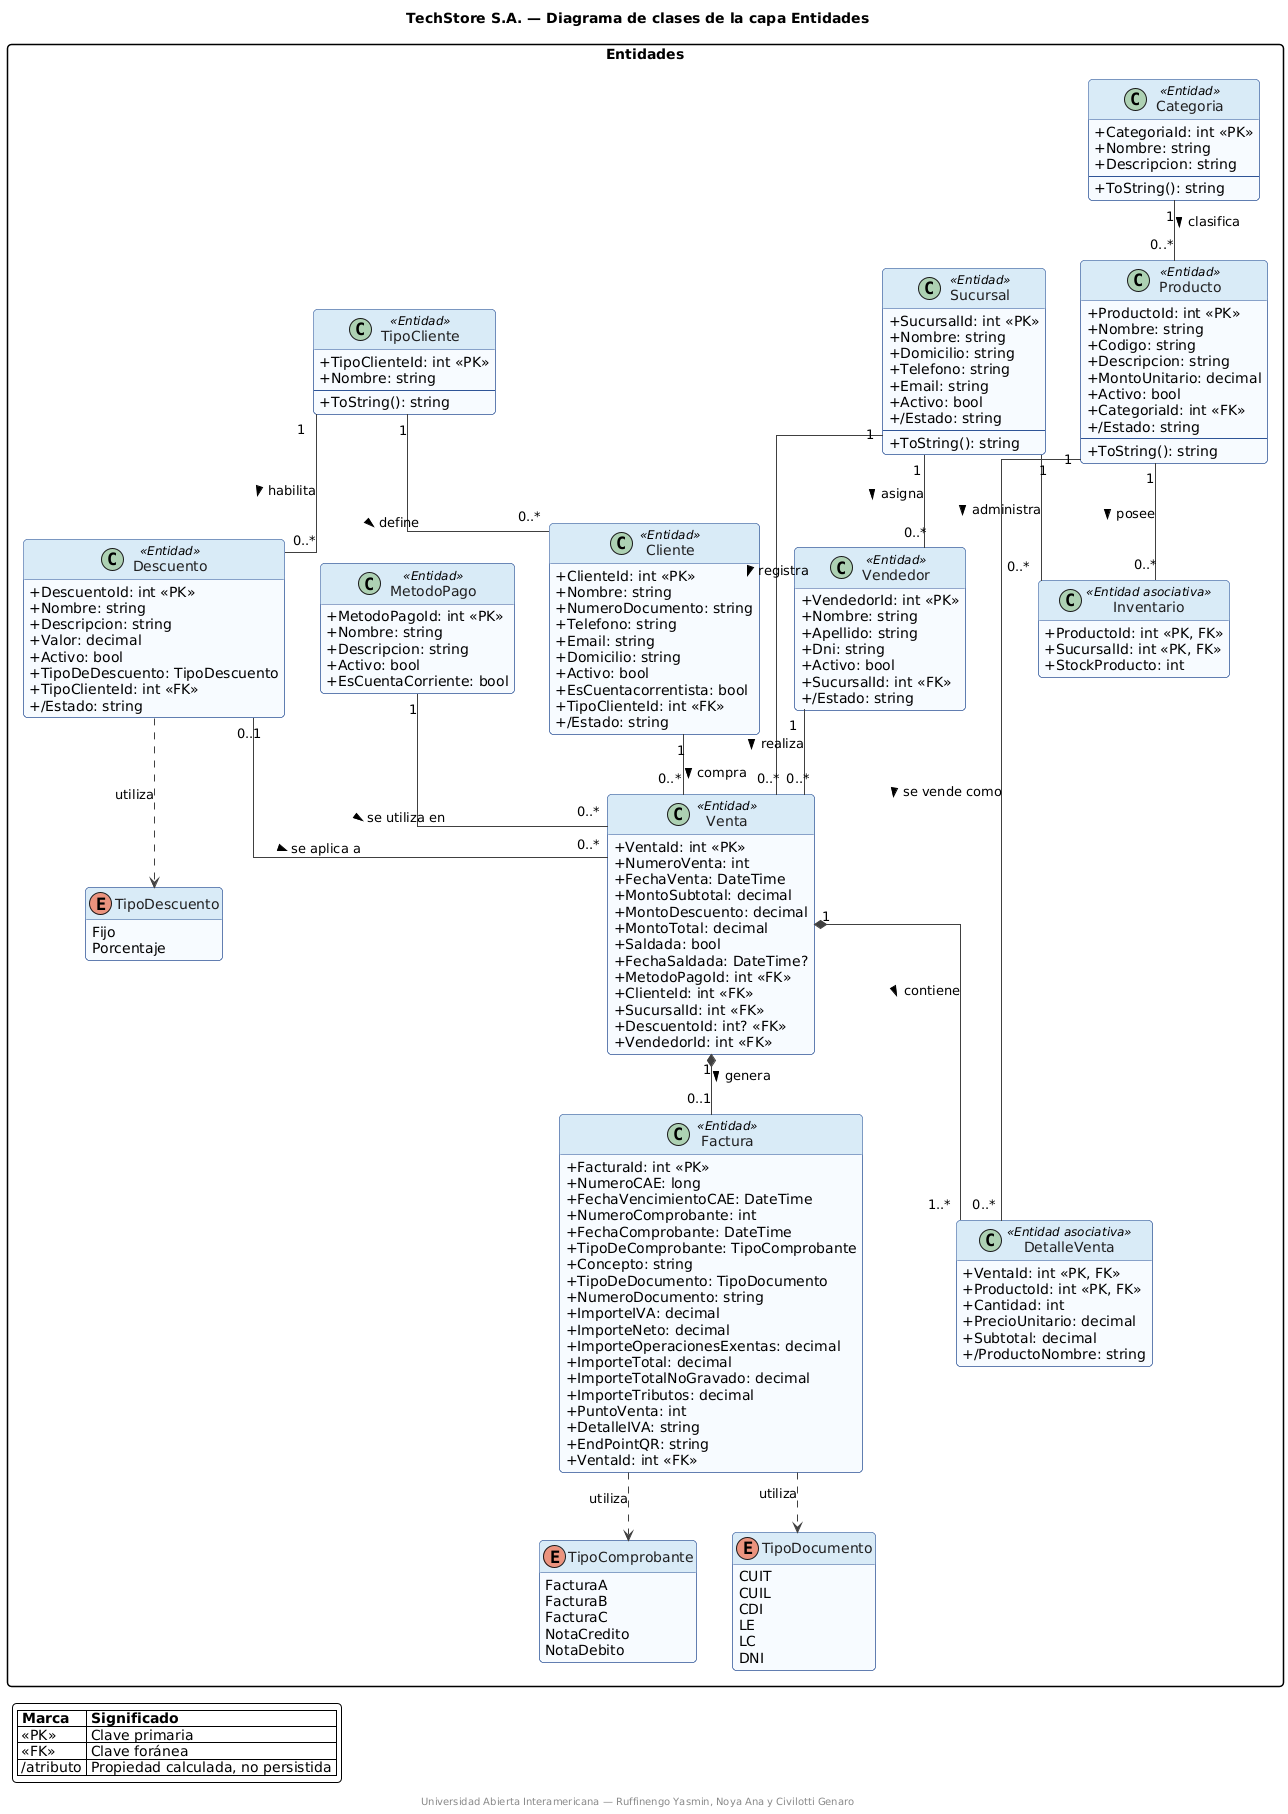
\includegraphics[
        width=\textwidth,
        height=0.80\textheight,
        keepaspectratio
    ]{DiagramaClases.png}
    \caption{Diagrama de clases de la capa Entidades}
    \label{fig:diagrama-clases-entidades}
\end{figure}

\end{document}
